%!TEX root = ../main.tex
\documentclass[../main]{subfiles}
\ifSubfilesClassLoaded{
    \addbibresource{../Biblio/biblio.bib}
    \dominitoc
    \tableofcontentsfile
    \pagenumbering{arabic}
    \setcounter{page}{1}
}{}
\begin{document}
\chapter{Méthodes de représentation et d'analyse de l'architecture CxSOM}
\graphicspath{{04-Representation/},{./figures/}}
\minitoc

\section{Introduction}

Dans le chapitre précédent, nous avons proposé l'algorithme CxSOM, permettant de construire des architectures non-hiérarchiques modulaires de cartes auto-organisatrices. 
Dans ces architectures non-hiérarchiques, plusieurs cartes sont connectées. 
Chaque carte a pour but d'extraire une représentation de ses entrées externes, tout en prenant comme entrée secondaire les positions des \emph{Best Matching Unit} d'autres cartes afin de mettre en relation les activités relatives aux différentes modalités. 
La particularité du modèle CxSOM est d'introduire des rétroactions entre cartes: l'architecture n'est pas un empilement de cartes qui apprennent tour à tour, de façon ascendante.
Le but de ce modèle est à terme de pouvoir construire des architectures assemblant un grand nombre de cartes~; nous nous concentrons dans cette thèse sur des petites architectures de deux et trois cartes afin de comprendre les comportements qui émergent d'un tel système.

Nous étudions l'architecture CxSOM dans un cadre particulier de mémoire associative.
L'objectif pour une architecture de cartes est alors d'apprendre une représentation des relations existant entre des entrées de différentes modalités, tout en apprenant une représentation au sein de chaque carte d'un espace d'entrée.
La compréhension du comportement de structures avec un faible nombre de cartes posera des bases pour la construction d'architectures plus grandes. Ce système de cartes est un système complexe, même dans une architecture de quelques cartes. Chaque carte possède 500 unités~; son état, représenté par son BMU, peut alors prendre 500 valeurs et l'état d'une carte dépend des cartes voisines.

Cette thèse s'inscrit alors dans une démarche complètement expérimentale d'étude d'un système complexe~: nous observerons l'organisation d'architectures de cartes sur différents espaces d'entrées et différentes configurations et observerons comment l'organisation qui en émerge traduit l'apparition d'un phénomène de mémoire associative. 
Pour analyser l'organisation de ces cartes, nous aurons besoin de d'introduire de nouvelles représentations par rapport à l'étude d'une SOM classique. Nous voulons également poser un formalisme clair sur des architectures de quelques cartes pour permettre l'adaptation de CxSOM à plus grande échelle.

Nous posons ainsi dans ce chapitre la méthode expérimentale que nous utiliserons dans toutes les expériences présentées dans ce manuscrit. Nous y présenterons les représentations adaptées à cette méthode expérimentale ainsi que le formalisme utilisé. Ces représentations ont pour but non seulement de qualifier la qualité de l'apprentissage mais surtout de mettre en lumière les propriétés et l'organisation des cartes émergeant de l'algorithme d'apprentissage. 

\subsection{Présentation d'une expérience multimodale minimale illustrant les représentations}

La méthode expérimentale sera présentée dans toute ce chapitre sur l'exemple minimal d'une architecture de deux cartes. L'architecture est illustrée à droite en figure~\ref{fig:exp}~: elle est composée de deux cartes en une dimension. Chaque carte prend une entrée externe. Il s'agit de $\inpx\m{1}=x$ et $\inpx\m{2}=y$, les coordonnées de points 2D sur un cercle. Ces deux modalités sont dépendantes~: pour une valeur de $x$, seule deux valeurs sont possibles pour $y$, et symétriquement. Les entrées sont représentées sur le schéma de gauche, figure~\ref{fig:exp}.
Ces entrées externes sont normalisées entre 0 et 1. Les points sont donc sur un cercle de centre $x_c,y_c = 0.5,0.5$ et de rayon $0.5$.
Les deux cartes sont des lignes 1D de 500 n\oe{}uds. Les rayons de voisinage sont $h_e = 0.2$ et $h_c = 0.02$.
Chacune des deux cartes est également connectée à sa voisine, c'est-à-dire, la carte $M\m{1}$ prend en entrée contextuelle la position du BMU de $M\m{2}$, et inversement.
%es données relatives à cette expérience et le code permettant de faire les tracés sont fournies sur git.
Afin de comprendre les tracés que nous présenterons, nous utiliserons deux cartes de Kohonen 1D classiques en tant que témoin.
Ces cartes prennent en entrée les valeurs $x$, et la deuxième les valeurs $y$, mais sans être connectées entre elles. Il s'agit de cartes classiques, prendant une entrée. Les paramètres de ces cartes sont les mêmes que les cartes de CxSOM: 500 n\oe{}uds, de rayon de voisinage constant $h_e = 0.2$.

\begin{figure}
\begin{minipage}{0.4\textwidth}
\centering
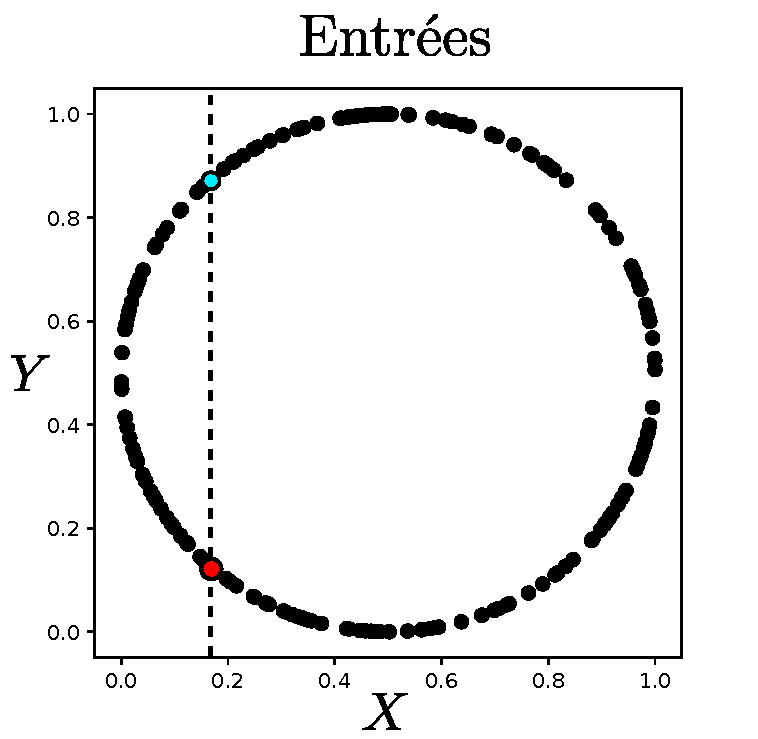
\includegraphics[width=0.8\textwidth]{2som_inp_noinformation}
\end{minipage}
\begin{minipage}{0.6\textwidth}
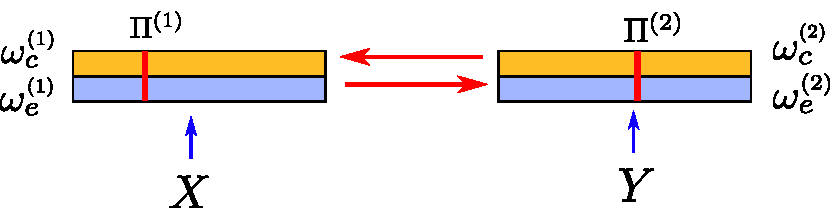
\includegraphics[width=\textwidth]{2som_archi}
\end{minipage}
\caption{A gauche, disposition des entrées dans l'exemple illustratif, sous forme de cercle. A droite, l'architecture de deux cartes en une dimension utilisée sur ces entrées dans ce chapitre pour illustrer les méthodes de représentation.\label{fig:exp}}
\end{figure}

\subsection{Représentations et indicateurs classiques des cartes de Kohonen}

Les cartes de Kohonen sont particulièrement associées à une facilité de représentation et de visualisation. Leur nombre réduit de prototypes et leur aspect topologique permet d'en tracer une représentation visuelle interprétable.
La manière la plus couramment utilisée de représenter une carte de Kohonen est de tracer les poids de ses prototypes, disposés dans le graphe (ligne ou grille) qu'est la carte. Deux exemples courants de représentation sont les suivants: 
\begin{itemize}
\item Le graphe qu'est la carte de Kohonen est représenté dans l'espace de ses positions (la grille d'indices $(i,j)$, ou une ligne indexée par $i$. Sur chaque noeud est tracé le poids correspondant. C'est le cas sur l'exemple de gauche en figure~\ref{fig:representation} dans lequel les poids des prototypes, qui sont des imagettes, sont affichés en chaque point de la grille. 
\item Lorsque les données traitées sont des points deux ou trois dimensions, les poids des prototypes peuvent être directement tracés dans l'espace $\mathbb{R}^2$ ou $\mathbb{R}^3$. Ces poids sont reliés en fonction des positions des n\oe{}uds dans la carte, montrant ainsi la déformation de la carte dans l'espace d'entrée, c'est le cas sur l'exemple de droite en figure~\ref{fig:representation} pour une grille en deux dimension.
\end{itemize}

Nous utiliserons des représentations adaptées au cas d'une architecture à plusieurs cartes à partir de ces deux modes de représentation. 
Cette adaptation dans le cas précis d'une architecture CxSOM est l'objet de cette section.

\begin{figure}
\begin{minipage}{0.5\textwidth}
\centering
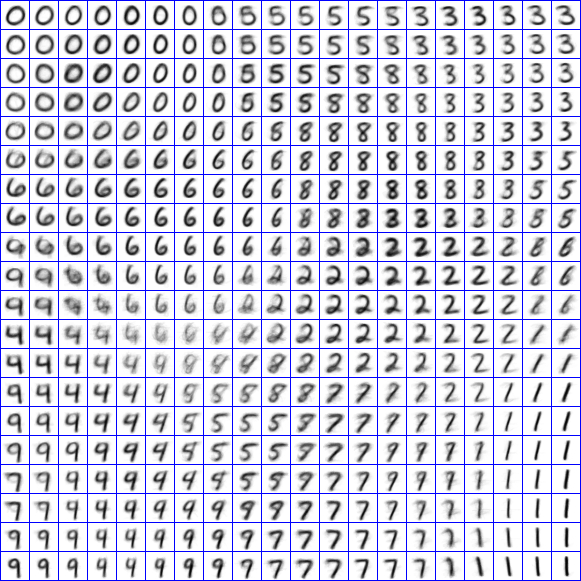
\includegraphics[width=0.5\textwidth]{digits.jpg}
\end{minipage}
\begin{minipage}{0.5\textwidth}
\centering
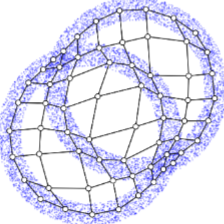
\includegraphics[width=0.5\textwidth]{points.png}
\end{minipage}
\caption{Représentations possible des poids d'une carte de Kohonen classiques, dans le cas d'entrées sous forme d'imagettes ou de points en deux dimensions.\label{fig:representation}}
\end{figure}

\subsection{Limites des représentations classiques dans le cas d'une architecture CxSOM}

Utilisons d'abord les représentations classiques mentionnées ci-dessus pour tracer les poids de chacun des cartes d'une architecture CxSOM à la fin de l'apprentissage.
La fin de l'apprentissage est définie comme le moment où les poids ont convergé vers une organisation restant stable au cours des itérations $t$.
La figure~\ref{fig:weights} présente le tracé des poids des deux cartes de l'exemple.
La courbe orange correspond aux poids externes des cartes, se dépliant sur chaque coordonnée $\inpx\m{1} = x$ et $\inpx\m{2} = y$ des points du cercle, appartenant chacune à $[0,1]$.
Ce tracé permet d'observer que les poids externes couvrent l'intervalle $[0,1]$, et sont organisés de façon monotone: ce comportement est celui qu'on attend dans une carte de Kohonen classique. Les poids contextuels, en bleu, ne présentent pas cette organisation monotone. Ils présentent toutefois une continuité: deux prototypes proches ont des poids proches. Le tracé des deux couches de poids nous informe donc sur le caractère continu de l'organisation de chacune de couches de poids. 

Notons que nous ne pouvons pas en tirer plus de conclusion: la représentation des poids de la figure~\ref{fig:weights} ne différencie pas les n\oe{}uds qui seront effectivement BMUs, des n\oe{}uds dits \emph{morts}.
Ces n\oe{}uds morts ont bien un poids, mais ne seront jamais BMUs.
Dans une carte de Kohonen classique, ces n\oe{}uds correspondent à des transitions, liant deux zones denses de l'espace d'entrée séparées par une zone sans points.
Par ailleurs, cette représentation concerne une seule carte. Nous ne pourrons pas tirer de conclusion sur l'influence des connexions entre cartes à partir de cette seule représentation.

Au regard des insuffisances des représentations classiques, que nous avons révélées sur un cas très simple de deux cartes mono-dimensionnelles, nous constatons qu'il est nécessaire de trouver un moyen de représenter l'architecture comme un tout. Nous devons ainsi définir des représentations qui montrent comment l'architecture de cartes est capable d'apprendre les relations entre les entrées multimodales.

\begin{figure}
\centering
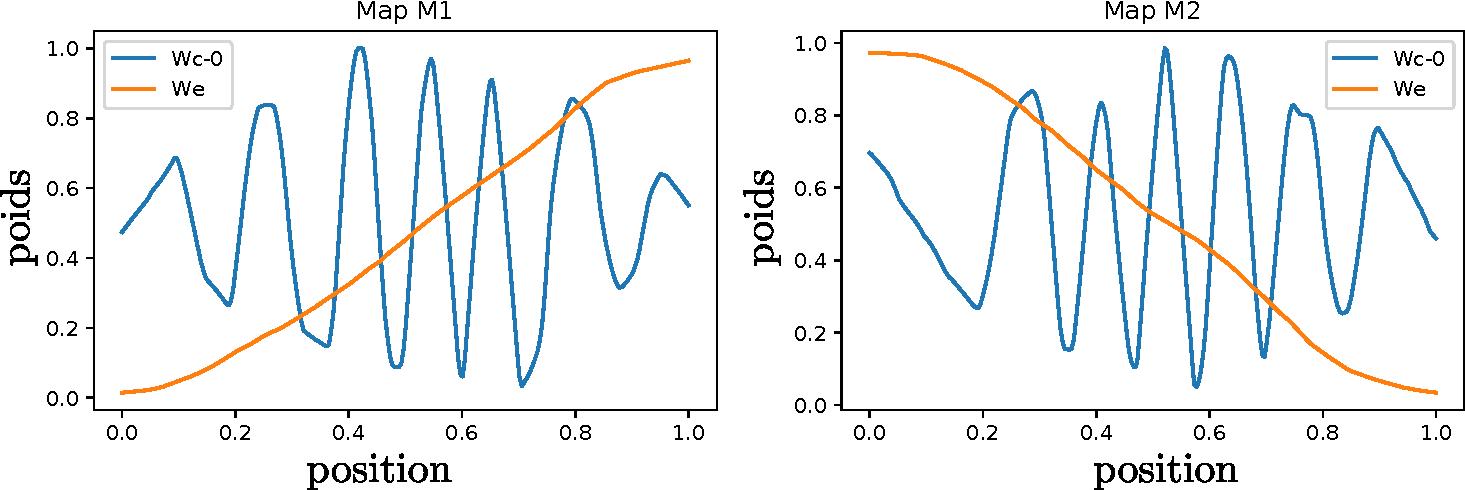
\includegraphics[width=0.9\textwidth]{weights_cercle1.pdf}

\caption{Représentation des valeurs des poids d'une carte au sein de CxSOM après apprentissage en fonction de leur position dans la carte. La seule représentation de ces poids ne suffit pas à savoir comment la carte se comporte.\label{fig:weights}}
\end{figure}

\subsection{Problématique}

Suite aux limites montrées par les méthodes de représentation classiques utilisées dans le domaine des SOMs, ce chapitre propose plusieurs façons de représenter une carte au sein d'une architecture.
Nous présenterons en premier lieu le formalisme décrivant les cartes et leurs entrées multimodales associées ainsi que la méthode expérimentale que nous utiliserons pour toutes les expériences présentées dans cette thèse. \'A partir de ce formalisme, nous proposerons plusieurs représentations permettant de comprendre et représenter ce que calcule une architecture CxSOM sur les données d'entrées. Ces représentations seront illustrées sur un exemple minimal de deux cartes pour faciliter la compréhension. Nous utiliserons ces méthodes dans les chapitres suivants pour analyser le comportement des cartes.

\section{Formalisation statistique des entrées et sorties des cartes}

Nous introduisons dans cette section un formalisme traitant les éléments des cartes et les entrées en tant que variables aléatoires. 
Ce formalisme possède à la fois l'avantage de clarifier les représentations et de permettre le développement d'indicateurs statistiques sur l'apprentissage effectué par les cartes.

\subsection{Formalisation des entrées}

Plaçons nous dans le cas général d'une architecture de $N$ cartes pour formaliser davantage.
Nous considérons des entrées multimodales tirées d'un ensemble d'espaces d'entrée $\mathcal{D}\m{1},\cdots,\mathcal{D}\m{n}$. Chaque espace $\mathcal{D}\m{i}$ est une modalité.
Les observations multimodales que l'on cherche à apprendre par l'architecture de cartes sont notées $(\inpx\m{i} \in \mathcal{D}\m{i}, i = 1 \cdots N)$.
Nous choisissons de modéliser ces entrées $\inpx\m{i}$ comme des \emph{variables aléatoires}.
Chaque variable aléatoire possède une distribution $p\m{i}$ sur $\mathcal{D}\m{i}$.
Nous notons $\mathbf{\inpx} = (\inpx\m{1}, \cdots, \inpx\m{n})$ la variable aléatoire jointe.
Cette variable appartient à l'espace $\mathcal{D}\m{1} \times \cdots \times \mathcal{D}\m{n}$.
A chaque pas de temps, un vecteur $\mathbf{\inpx} = (\inpx\m{1}_t, \cdots , \inpx\m{n}_t)$ est présenté à l'architecture: il s'agit d'une réalisation de la variable jointe $\mathbf{\inpx}$. 

En pratique, ces variables sont des observations, issues par exemple de capteurs d'un robot. Ces observations sont issues d'un environnement général et sont donc liées par des relations au sein de ce modèle d'environnement~: les variables $\inpx\m{i}$ ne sont pas des variables indépendantes.
Nous introduisons la notion de \emph{modèle d'entrées} se rapportant à cette dépendance entre variables.
Le modèle d'entrée fait référence au modèle d'environnement permettant de générer les entrées multimodales fournies en entrées. Dans l'exemple d'illustration, les modalités sont les abscisses $\inpx\m{1} = x$ et les ordonnées $\inpx\m{2} = y$; le modèle d'entrées correspond au cercle, modélisé par une équation.

Le but de l'apprentissage non-supervisé par des cartes de Kohonen classiques est d'apprendre une représentation discrète de l'espace d'entrée.
Avec CxSOM, nous chercherons à la fois à apprendre un représentation discrète des espaces d'entrée mais aussi à apprendre une représentation du modèle d'entrées.

Les tracés que nous développerons dans cette section ont pour but de mesurer comment ce modèle d'entrées est représenté par l'architecture. 

\subsection{Formalisation du modèle d'entrée par une variable cachée}

Nous cherchons à évaluer expérimentalement la capacité du modèle CxSOM à apprendre à partir d'un environnement multimodal. Dans ce cadre expérimental particulier, nous choisissons des modèles d'entrées dont les relations sont connues.
Ces modèles peuvent être paramétrisés par une variable multidimensionnelle $U$. Les modalités sont alors définies comme des fonctions de cette variable:
$\inpx\m{i} = f\m{i}(U)$
$U$ est une nouvelle variable aléatoire représentant le modèle.

Pour que la variable $U$ conserve toute l'information sur le modèle d'entrées, la fonction $(f\m{1}, \cdots, f\m{n})$ : $(\inpx\m{1}, \cdots \inpx\m{n})\rightarrow U$ doit être une bijection. Toute valeur d'entrées jointes correspond à un seul $U$, toute valeur de $U$ renvoie à une seule valeur d'entrées jointes. 
La définition de $U$ peut aussi être considérée comme un cas particulier de réduction de dimension du modèle, dans lequel la variable $U$, de dimension plus faible que $\mathbf{X}$, réduit la dimension des entrées sans perte d'information.

Dans le cas d'exemple, $\mathbf{X} = (\inpx\m{1},\inpx\m{2})$ est un vecteur aléatoire prenant comme valeurs les coordonnées cartésiennes des points du cercle de centre $x_c,y_c = 0.5,0.5$ et de rayon $r = 0.5$.
En définissant une variable $U$ scalaire à valeurs dans $[0,1]$, ces variables aléatoires peuvent maintenant s'écrire, selon l'équation paramétrique du cercle:
\begin{equation}
 \begin{cases}
     \inpx\m{1}= x_c + r  \cos(2\pi U)\\
     \inpx\m{2} = y_c + r \sin(2 \pi U)
    \end{cases}\,.
\end{equation}

$U$ représente ici l'angle du point sur le cercle (à un facteur $2\Pi$ près).
Ce modèle n'étant pas fourni à l'architecture de cartes lors de l'apprentissage, il s'agit d'un modèle \emph{latent}.
Nous cherchons, par l'architecture de cartes, à apprendre les entrées et les relations entre entrées: nous cherchons donc à extraire une structure dans le modèle latent. La relation entre $U$ et $\mathbf{X}$ est bijective; de ce fait, étudier comment l'architecture de cartes a appris $U$ est équivalent à étudier comment l'architecture a appris le modèle d'entrées.

Cet exemple est scalaire mais la représentation sous forme de variable cachée est générale à n'importe quel dimension et nombre d'entrées. En effet, toute configuration d'entrée multimodale dépend d'un environnement global. La variable $U$ correspond alors aux paramètres de cet environnement. Néanmoins, dans le cas de variables non artificielles, cette variable d'environnement est inconnue.
Nous utiliserons donc la variable cachée $U$ uniquement dans les expériences sur données artificielles. Elle nous permettra d'étudier et de représenter comment les cartes apprennent le modèle d'entrées.

\begin{figure}
\centering
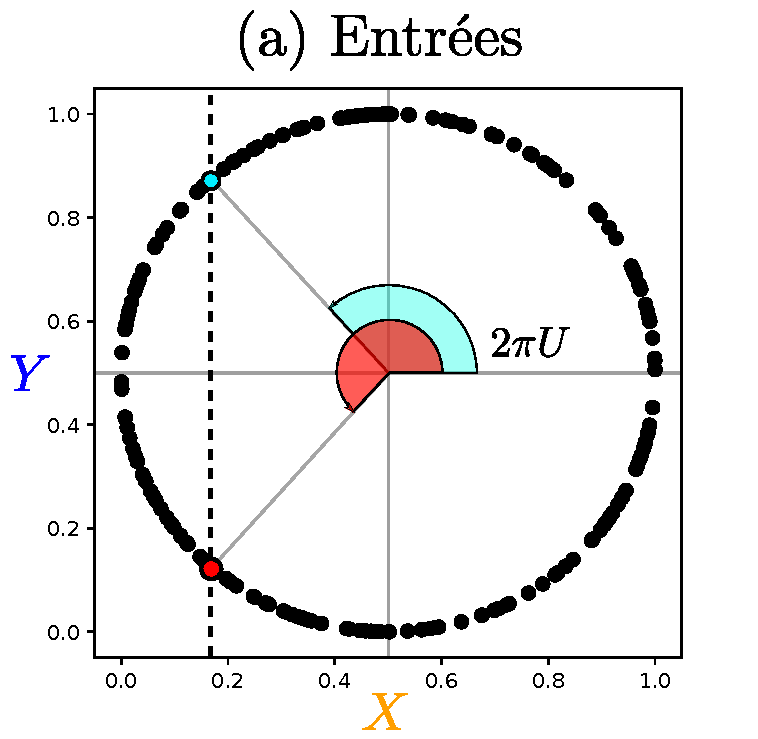
\includegraphics[width=0.4\textwidth]{2som_inp.pdf}
\caption{Représentation choisie pour le cercle. Le modèle auxquelles appartiennent les modalités $\inpx\m{1}$ et $\inpx\m{2}$ est représenté par la variable $U$. \label{fig:U}}
\end{figure}


\subsection{Démarche expérimentale}

Afin d'étudier le comportement de la carte à n'importe quel instant $t$ de l'apprentissage, nous effectuons une phase de \emph{test}, décrit en figure~\ref{fig:flowchart}.
Lors de cette phase de test, des entrées sont présentées à la carte, mais seul le processus de recherche de la best matching unit est réalisé, les poids des cartes ne sont pas mis à jour. Cet étape génère un ensemble de réponses de la carte aux entrées présentées.
Les entrées utilisées lors du test sont un échantillon de taille 1000 de la variable aléatoire $(\inpx\m{1}, \cdots, \inpx\m{n})$.
La distribution des entrées test est identique à la distribution des entrées d'apprentissage ayant servi au dépliement de la carte.

Nous formalisons non seulement les entrées mais aussi chaque élément de réponse des cartes d'une architecture comme une variable aléatoire.
Un élément de réponse d'une carte est une valeur régissant aux entrées lors d'une itération: positions du BMU, activité, poids du BMU.
Nous choisissons notamment de s'intéresser aux position des BMUs $\bmu\m{1}, \cdots, \bmu\m{n}$ et à leurs poids $\w\ext\m{1}(\bmu\m{1})$ et $\w\ext\m{2}(\bmu\m{2})$.
La valeur de ces éléments est indépendante entre deux itérations de test, car les poids ne sont pas mis à jour.
Grâce à cette indépendance entre itérations, les valeurs obtenues lors d'une phase de test forment un échantillon de la variable aléatoire jointe : 
$$(\underbrace{\inpx\m{1}, \cdots, \inpx\m{n}, U,}_{\text{Entrées}} \underbrace{\bmu\m{1}, \cdots, \bmu\m{n}, \w_e\m{1}(\bmu\m{1}), \cdots, \w_e\m{n}(\bmu\m{n})}_{\text{Eléments de réponse}})$$

Les composantes de cette variable jointe ne sont pas indépendantes. Maintenant que la démarche expérimentale est formalisées, les représentations présentées par la suite sont simplement des tracés de dépendances au sein d'un échantillon de test entre composantes de la variable jointe définie ci-dessus.

Les variables d'entrées sont à valeurs continues et $\bmu$ à valeurs discrètes, correspondant aux 500 n\oe{}uds d'une carte. Nous considérerons cependant $\bmu$ comme une variable continue plutôt qu'une grandeur discrète. En effet, l'ensemble des positions du BMU correspondent à une discrétisation de l'espace continu $[0,1]$, et sont ordonnées. Le déplacement par relaxation n'est pas limité aux positions discrètes des BMUs. Les variables aléatoires considérées sont bien à valeurs continues. Le formalisme par variable aléatoires permettra aussi d'utiliser des outils et métriques issus de la théorie de l'information pour qualifier l'organisation des cartes au sein de l'architecture, ce que nous ferons dans le chapitre~\ref{chap:indicateur}.

\begin{figure}
\centering
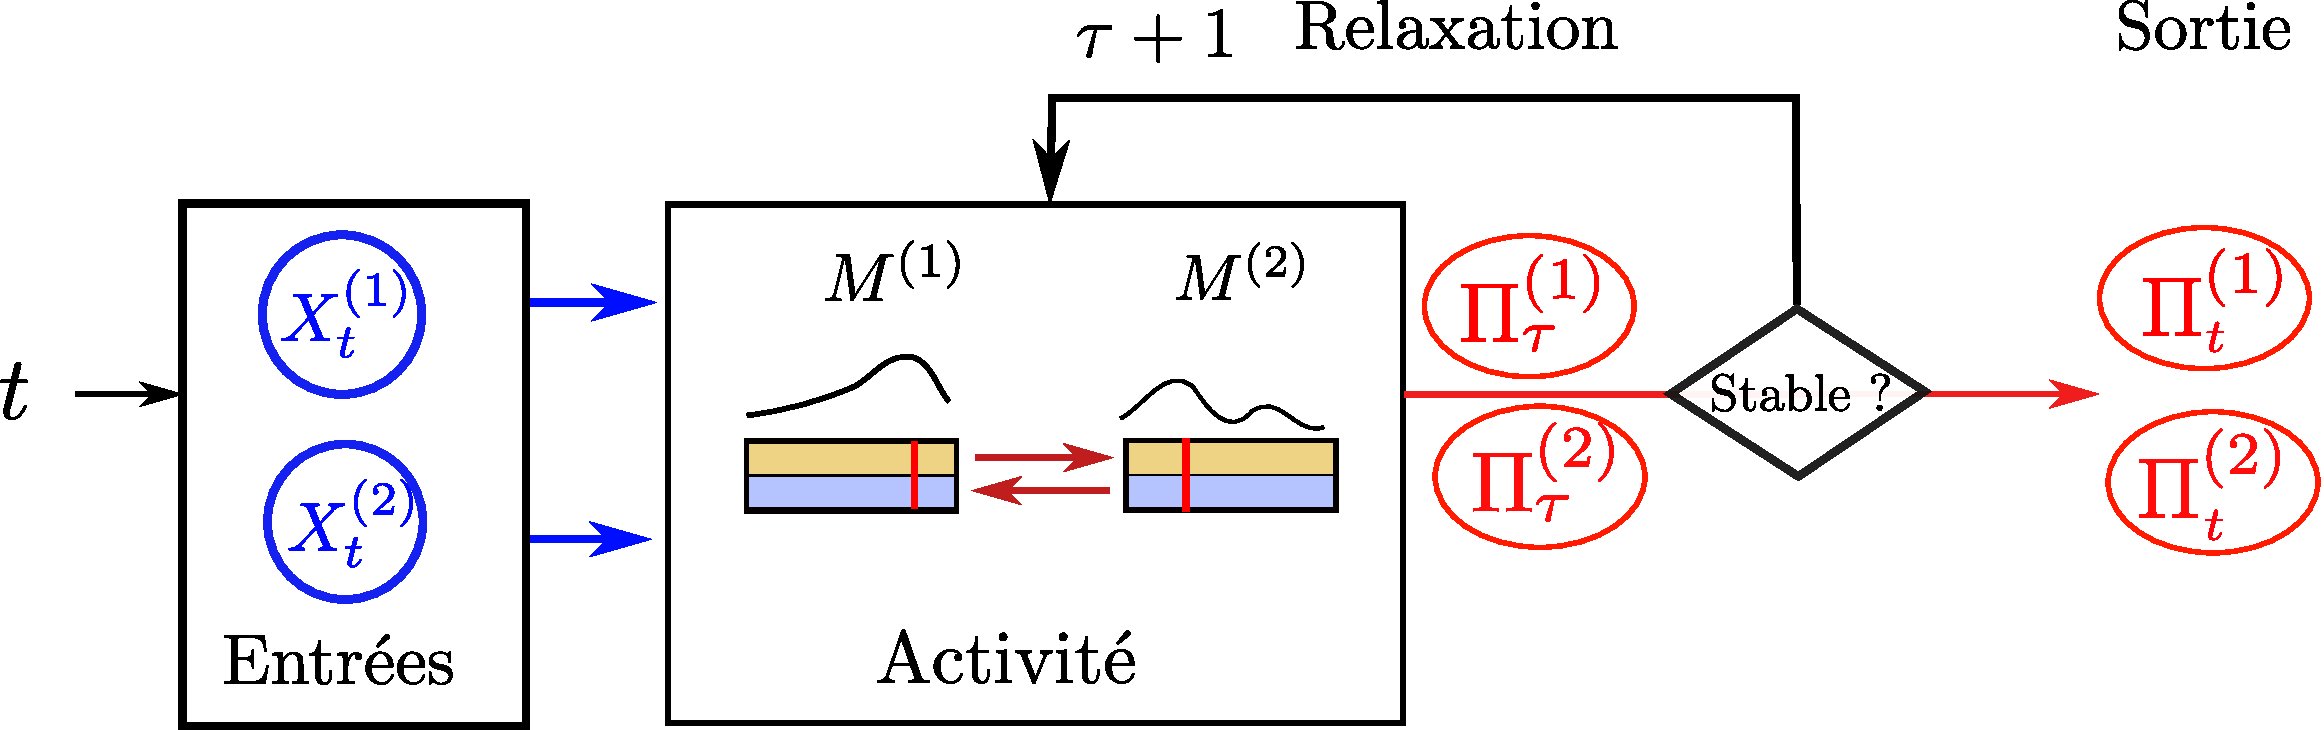
\includegraphics[width=0.85\textwidth]{tests_2maps.pdf}
\caption{Schéma décrivant une étape de test. Un test consiste à présenter successivement des réalisations de $\mathbf{X}$, notées $(\inpx\m{1}_t,\inpx\m{2}_t)$. Nous laissons le processus de relaxation stabiliser les BMUs. Quand la stabilité est atteinte, la valeur des positions de BMU $\bmu\m{1}_t$ et $\bmu\m{2}$ est obtenue. Un échantillon de test complet est ainsi obtenu en présentant un ensemble de réalisations de $\mathbf{X}$. Les poids ne sont pas mis à jour entre chaque itération, ce qui permet de considérer une phase de test comme un échantillonnage de la variable aléatoire $()\inpx\m{1},\inpx\m{2}, U, \bmu\m{1}, \bmu\m{2}$) }
\label{fig:flowchart}
\end{figure}

\section{Représentations graphiques}
A partir des échantillons de test, nous proposons dans cette section les représentations graphiques que nous utiliserons pour évaluer expérimentalement les architectures de cartes.
Ces représentations sont toute un tracé de dépendances entre des composantes de la variable $$(\inpx\m{1}, \cdots, \inpx\m{n}, U, \bmu\m{1}, \cdots, \bmu\m{n}, \w_e\m{1}(\bmu\m{1}), \cdots, \w_e\m{n}(\bmu\m{n}),U)$$ dont un échantillon est obtenu lors du test.
Nous proposons d'abord une représentation pour évaluer la qualité de quantification vectorielle effectuée par une carte de l'architecture. Nous présenterons ensuite des représentations nous permettant de comprendre comment le modèle d'entrées est appris par l'architecture CxSOM.

\subsection{Erreur de quantification d'une modalité dans chaque carte}

La première fonction d'une carte de Kohonen est de réaliser une tâche de quantification vectorielle sur son entrée externe. Au sein d'une architecture de cartes, nous nous attendons à ce que chaque carte extraie une représentation de la modalité qu'elle prend en entrée externe.
Afin de mesurer cette qualité de quantification vectorielle au sein d'une carte dans CxSOM, nous traçons le nuage de points correspondant au poids externe du BMU $\w_e(\bmu\m{i})$ en fonction de l'entrée externe présentée $\inpx\m{i}$. Une carte effectue une quantification vectorielle correcte si ce nuage de points est proche de la fonction identité.
Ces tracés sont réalisés en figure~\ref{fig:erreur} pour l'expérience exemple. Ces tracés s'approchent de l'identité: la quantification des entrées est correctement réalisée.
On pourrait mesurer une erreur quadratique moyenne pour déterminer numériquement cette erreur de quantification mais la représentation en nuage de points est, à défaut d'être quantitative, plus qualitative. En effet, ici, on observe que le nuage montre une structure "filamenteuse". Nous reviendrons sur ce point par la suite, nous contentant de souligner ici que la représentation graphique exprime une propriété que la simple mesure d'erreur n'aurait pas mise en évidence. 

Cette représentation nous informe ainsi sur la qualité de quantification dans une seule carte relativement à une seule modalité. Cette seule représentation est insuffisante à elle seule pour comprendre plus en détail le comportement d'une architecture de cartes: il nous faut également définir des méthodes de représentation permettant d'évaluer comment la structure globale du modèle d'entrées est apprise par l'architecture dans son ensemble.

\begin{figure}
    \centering
    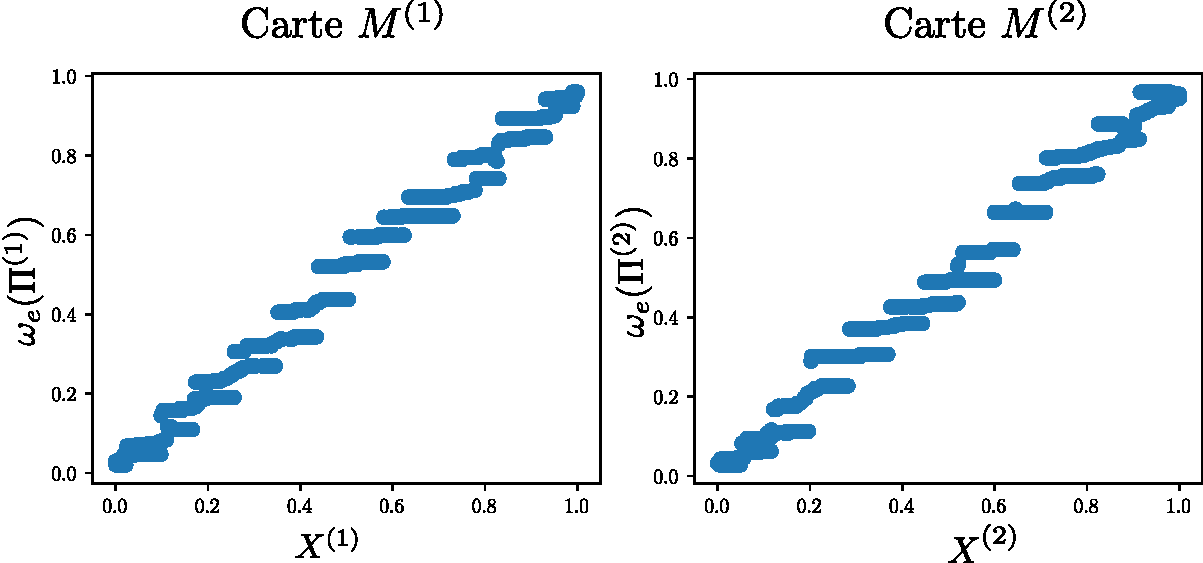
\includegraphics[width=0.7\textwidth]{w_x.pdf}
    \caption{Poids du BMU dans chaque carte en fonction de l'entrée présentée. On s'attend à des tracés proches de l'identité, montrant que le poids du BMU d'une carte est une bonne représentation de l'entrée. Sur ce graphique, on se rapproche effectivement de la fonction identité, cependant, une faible erreur est observée. On observe également un découpage des poids en bandes.\label{fig:erreur}}
\end{figure}


\subsection{Représentation cartographique des valeurs d'entrées préférentielles des BMUs}

En biologie, les aires du cortex cérébral sont cartographiées en faisant varier le motif d'entrée dans son espace, et en indiquant pour chaque neurone la valeur d'entrée préférentielle à laquelle il réagit. Cela donne alors une représentation cartographique où des valeurs de l'espace d'entrée sont tracées par rapport à la position sur le substrat neuronal du neurone qui y réagit.
Par exemple, une carte corticale est tracée pour l'aire visuelle primaire du cortex cérébrale, l'aire v1, en figure~\ref{fig:v1_repr}.

Un échantillon test donne un ensemble de valeurs de variable jointe $(\inpx\m{1}, \cdots, \inpx\m{n}, \bmu\m{1},\cdots, \bmu\m{n})$.
Dans la même idée que les cartes corticales, nous tracerons à partir de l'échantillon de test le nuage de points correspondant à la valeur de l'entrée $\inpx\m{i}$ d'une carte par rapport à la position du BMU $\bmu\m{i}$.
Cette représentation permet d'analyser la quantification des entrées par la carte. 
On s'attend à ce que les points soient proches de la courbe des poids externes de la carte $M\m{i}$.
Ce tracé fait également apparaître les zones dans lesquelles les neurones ne sont jamais best matching unit, les \emph{zones mortes}.
En plus des couples $(\bmu\m{i},\inpx\m{i})$, nous traçons également les entrées externes des autres cartes en fonction de $\bmu\m{i}$ : $(\bmu\m{i},\inpx\m{j})$.
Enfin, sur le même graphique, nous mettons ces valeurs d'entrées externes en relation avec les poids de la carte $M\m{i}$ en traçant les poids externes et contextuels de la carte $M\m{i}$ en fonction de leur position.
Une représentation cartographique fait ainsi apparaître les poids externes et contextuels d'une carte de l'architecture. A ces poids s'ajoutent plusieurs nuages de points correspondant aux valeurs d'une entrée $\inpx\m{j}$ en fonction du BMU de la carte $M\m{i}$, $\bmu\m{i}$.

En figure~\ref{fig:inputs}, nous avons ainsi tracé cette représentation cartographique pour l'exemple à deux cartes.
Nous y voyons deux nuages de points: $(\bmu\m{1},\inpx\m{1})$ et $(\bmu\m{1},\inpx\m{2})$ issus de l'expérience sur les deux cartes, ainsi que deux courbes: les poids externes et contexuels de la carte $M\m{1}$.
Deux valeurs issues de l'échantillon de test sont mise en évidence en couleur rouge et bleue sur chaque graphique. Un point de même couleur correspond à la même itération de test dans chaque graphique. Ces deux points partagent la même abscisse, donc l'entrée $\inpx\m{1}$ est la même pour ces deux échantillons. Par contre, leur ordonnée est différente: $M\m{2}$ reçoit donc une entrée $\inpx\m{2}$ différente entre de ces deux itérations.

Ce tracé nous permet d'abord d'observer que les points $(\bmu\m{1},\inpx\m{1})$ sont proches de la courbe de poids externe: le poids d'un BMU est proche de l'entrée qui a été présentée, le poids du BMU est donc une bonne approximation de cette entrée. Cela permet de conclure que la quantification vectorielle est bien réalisée dans cette carte sur les entrées externes, comme le montrait déjà la figure~\ref{fig:erreur}.

Tracer les échantillons de test permet ensuite d'observer la répartition des BMUs sur la carte. Les courbes de poids externes de la carte dans CxSOM (c) et de la carte indépendantes (b) sont indifférenciables; par contre, l'affichage de l'échantillon de test fait apparaître des zones mortes, sans BMUs. Nous observons ainsi que la carte au sein de CxSOM est découpée en plusieurs zones dans lesquelle les unités sont BMUs, séparées par des petites zones mortes. Ce tracé permet donc d'identifier un comportement nouveau dans une architecture de cartes, par rapport à une carte classique.

Les nuages de points $(\bmu\m{1},\inpx\m{1})$ et $(\bmu\m{1},\inpx\m{2})$ nous permettent d'observer quelles valeurs d'entrées sont codées dans les zones observées sur les positions des BMUs.
Nous observons notamment qu'une zone encode pour un intervalle de valeurs spécifique pour le couple $(\inpx\m{1},\inpx\m{2})$ et non seulement pour l'entrée externe de la carte, comme ce serait le cas dans une carte seule (b). Les points rouges et bleus illustrent ce comportement.
Ces échantillons correspondent à la même valeur d'entrée externe présentée à $M\m{1}$, mais $\inpx\m{2}$ est différent.
Dans la carte indépendante, le BMU sera identique pour ces deux valeurs.
Sur la figure (c), le point rouge et le point bleu ont leurs BMUs dans deux zones adjacentes, mais séparées, sur la carte.

La représentation des valeurs d'entrées $\inpx\m{j}$ selon la position du BMU $\bmu\m{i}$ permet ainsi d'identifier une répartition des BMUs sur une carte que nous ne pourrions pas observer en traçant simplement les poids.
Nous voyons notamment que la carte s'auto-organise en zones de BMUs, séparées par des zones mortes.
Les n\oe{}ds d'une zone réagissent à des valeurs spécifiques du couple d'entrées et non de seulement l'entrée externe.
Cette organisation en zone observée sur ce graphique traduit l'existence de deux échelles d'indices: une organisation primaire selon la valeur de l'entrée externe, et une organisation secondaire au sein des zones selon la valeur de l'entrée de l'autre carte.
Nous étudierons dans les chapitres suivants, grâce à cette représentation, si ce comportement se généralise pour différentes architectures et distributions d'entrées.

% Sur la figure (c), les BMUs appartenant à une même zone encodent les entrées $\inpx\m{1}$ ainsi que $\inpx\m{2}$ sur un intervalle particulier. Ce comportement diffère de celui de la carte simple (b). Dans cette carte, il n'y a pas de création de zones et un intervalle de position des BMUs encode deux intervalles distincts de valeurs concernant les entrées $\inpx\m{2}$.
% Les intervalles encodés par deux zones de BMUs adjacentes se recoupent: ce phénomène est illustré par le fait que les points rouges et bleus, ayant la même valeur de $\inpx\m{1}$, sont envoyés dans deux zones différentes.

% Ces valeurs peuvent être mises en relation avec celles de l'entrée $\inpx\m{2}$, également disposées selon $\bmu\m{1}$. Nous pouvons alors observer que deux zones adjacentes de la carte encodent des entrées proches selon $\inpx\m{1}$, mais très différentes pour $\inpx\m{2}$. Cela explique la séparation du point rouge et du point bleu dans deux zones.

\begin{figure}
    \centering
    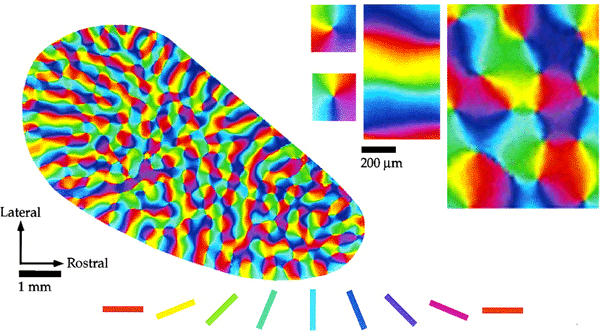
\includegraphics[width=0.7\textwidth]{v1.jpg}
    \caption{Carte corticale de l'aire cérébrale visuelle V1. Pour tracer cette représentation, un ensemble de traits de différentes orientation sont présentés en stimuli visuels au sujet, indiqués en bas de l'image. Le neurone réagissant à une entrée d'orientation particulière est coloré sur la carte de la couleur correspondante à l'entrée. Cette méthode permet de tracer des \emph{cartes corticales} d'une aire cérébrale \cite{Bosking1997OrientationSA}. \label{fig:v1_repr}}
\end{figure}

\begin{figure}
\begin{minipage}{0.27\textwidth}
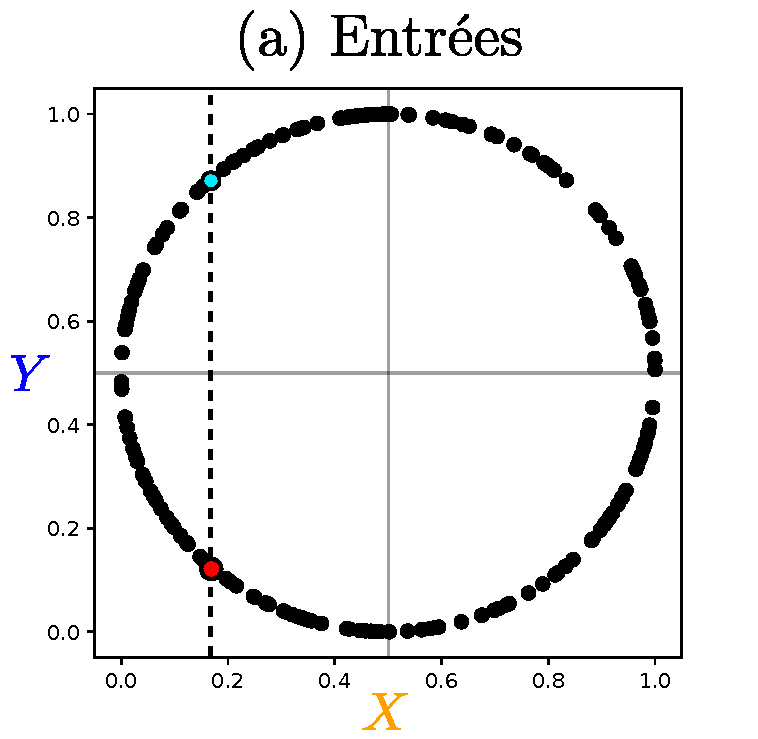
\includegraphics[width=\textwidth]{2som_inp_noU.pdf}
\end{minipage}
\begin{minipage}{0.34\textwidth}
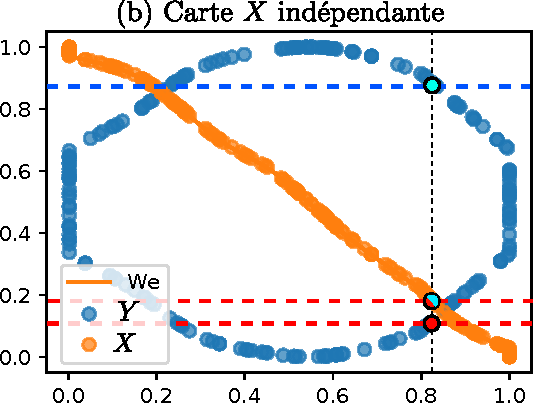
\includegraphics[width=\textwidth]{weights_2som_unco.pdf}
\end{minipage}
\begin{minipage}{0.38\textwidth}
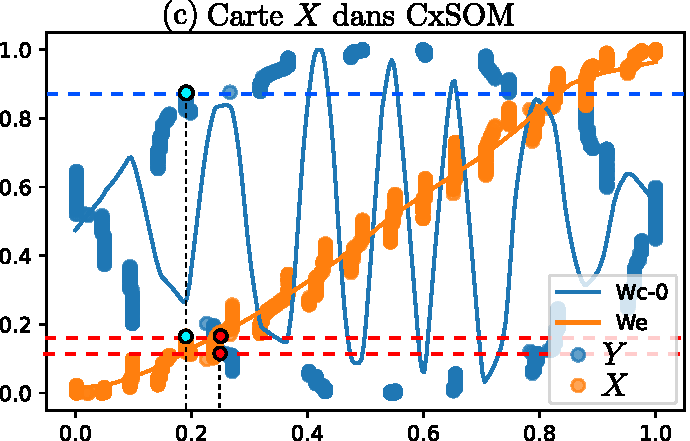
\includegraphics[width=\textwidth]{weights_2som.pdf}
\end{minipage}

\caption{Représentation des entrées $\inpx\m{1},\inpx\m{2}$ d'une architecture de deux cartes relativement au BMU de la carte $M\m{1}$ après apprentissage. Ces tracés mettent en valeur l'organisation des cartes, différentes dans le cas ou les cartes apprennent indépendemment leurs entrées~(b) ou sont connectées~(c). Les entrées correspondantes sont en figure~(a). Les points bleu et rouge reportés sur les tracés correspondent au même échantillon de test.\label{fig:inputs}}
\end{figure}

\subsection{Représentation de la variable cachée selon les positions des BMUs}

Nous avons vu lors de la représentation cartographique des entrées que chacune des cartes choisit son BMU  en fonction non seulement de son entrée externe, mais aussi de l'entrée de l'autre carte. Chaque carte s'organise donc en fonction du \emph{modèle d'entrée}, donc en fonction de $U$.
Afin de mettre en valeur ce comportement, nous tracerons les nuages de points représentant $U$ en fonction de la position $\bmu\m{i}$ du BMU d'une carte pour afficher comment la position du BMU traduit la relation entre les entrées.

En figure~\ref{fig:piu}, nous traçons $U$ en fonction de $\bmu\m{1}$ et $U$ en fonction de $\bmu\m{2}$.
Ce tracé montre $U$ comme une fonction de la position du BMU dans chaque carte, contrairement au cas ou les cartes ne sont pas connectées pour lequel deux valeurs de $U$ correspondent à un même BMU. Cela traduit bien le fait que chaque carte a appris une représentation du modèle d'entrée et non seulement de son entrée externe.
L'organisation de la carte dans CxSOM montre donc chaque position $\bmu$ codant pour une seule valeur de $U$, c'est à dire une seule position d'échantillon sur le cercle.
La représentation de $U$ selon la position du BMU d'une carte $\bmu\m{i}$ permet de représenter comment la carte $i$ a appris l'ensemble d'entrées $(\inpx\m{1},\inpx\m{2})$ et non seulement son entrée externe. Déterminer si l'architecture a appris le modèle d'entrées revient alors à vérifier si $U$ est une fonction de $\bmu$ dans chacune des cartes de l'architecture.

Cette représentation fait appararaître $U$ comme une fonction de $\bmu$ dans chaque carte. Ce comportement traduit le fait que les cartes s'organisent en fonction de tout le modèle d'entrée, non seulement de leur entrée externe. Il s'agit là d'un comportement que nous pouvons qualifier de comportement de base pour CxSOM. 

\begin{figure}
\centering
\includegraphics[width = 0.7\textwidth]{xu_yu_both.pdf}
\caption{Valeur de $U$ en fonction des valeurs du BMU $\bmu\m{i}$ dans chacune des cartes dans l'exemple d'illustration. Sur la première ligne, nous traçons la réponse de chaque carte à son entrée dans le cas ou les deux cartes ne sont pas connectées. Sur la deuxième ligne, nous traçons la réponse de chaque carte lorsqu'elles ont appris de façon jointe au sein de CxSOM.
$U$ apparaît alors comme une fonction de la position du BMU $\bmu\m{i}$ dans chaque carte, contrairement au cas ou les cartes apprendraient indépendamment sur les mêmes entrées. Cette relation fonctionnelle est symbolisée par les pointillés sur les tracés du bas. Les mêmes échantillons rouge et bleu mis en évidence en figure~\ref{fig:inputs} sont reportés sur les tracés.}
\label{fig:piu}
\end{figure}


\subsection{Dépliement d'une carte dans l'espace d'entrée multimodal}

Une représentation classique utilisée pour représenter une carte de Kohonen est de tracer les poids du graphe qu'est la carte dans l'espace de ses entrées, telle qu'en figure de droite en~\ref{fig:representation}. Dans CxSOM, chaque carte prend en entrée une seule des modalités. Par contre, grâce à l'échantillon de test, il est possible de représenter comment la carte se déplie dans l'espace de toutes les modalités.

Nous définissons alors une façon de représenter le dépliement d'une seule carte de CxSOM dans l'espace global des entrées. Dans l'exemple, il s'agit de représenter le dépliement de $M\m{1}$ dans l'espace des entrées $\inpx\m{1},\inpx\m{2}$.
Au lieu de s'appuyer sur les poids des cartes comme en~\ref{fig:representation}, nous utilisons les valeurs de l'échantillon de test. Nous traçons le nuage de poids correspondant au poids des BMUs: $\w_e\m{1}(\bmu\m{1},\w_e\m{2}(\bmu\m{2})$, puis relions ces points selon l'ordre de leurs positions dans la carte $M\m{1}$ ou $M\m{2}$. Ainsi, nous obtenons une représentation des cartes $M\m{1}$ ou $M\m{2}$ dépliées dans l'espace global des entrées. 
Notons que les unités mortes ne peuvent pas être représentées sur la carte. Nous ne représentons que les morceaux de cartes étant effectivement BMUs. 
Cette représentation est tracée en ~\ref{fig:distortion} pour l'exemple à deux cartes.


La carte représentant les poids externes des BMUs, on s'attend à ce que la forme du nuage de points corresponde à la structure des entrées.
Les tracés mettent en lumière les propriétés observées lors de la représentation cartographique des entrées, à savoir l'apparition de zones dans chaque carte. Les poids suivent la structure circulaire des entrées en découpant l'espace en zones. Les parties du cercle effectivement représentées par les poids sont réduites: le cercle est comme discrétisé en petits morceaux.
Dans l'exemple, on remarque la façon dont est parcouru l'espace dans chaque carte: en fonction de $x$ dans la carte $M\m{1}$, et en fonction de $y$ dans la carte $M\m{2}$. 
Cette représentation offre la possibilité  de visualiser comment une carte se déplie dans l'espace d'autres modalités.

\begin{figure}
    \begin{minipage}{0.49\textwidth}
    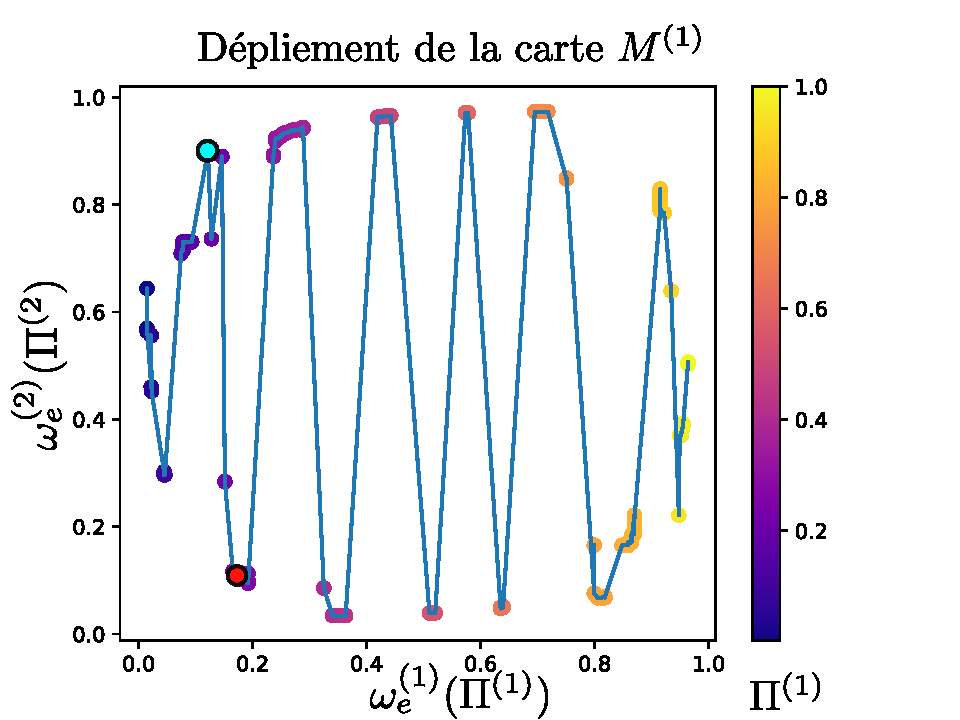
\includegraphics[width=\textwidth]{disto_cercle_M1.pdf}
    \end{minipage}
    \begin{minipage}{0.49\textwidth}
    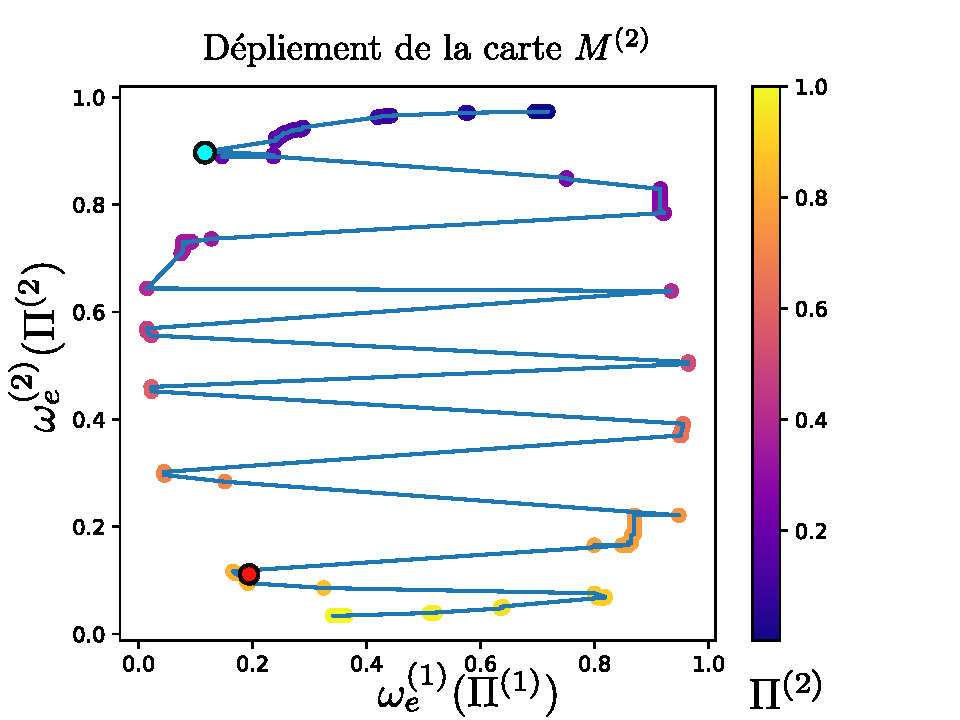
\includegraphics[width=\textwidth]{disto_cercle_M2.pdf}
    \end{minipage}
    \caption{Dépliement des cartes $M\m{1}$ et $M\m{2}$, reliés dans l'ordre de leurs positions selon $M\m{1}$ figure de gauche et $M\m{2}$ figure de droite. Le dépliement de chacune des cartes est alors représenté dans l'espace complet des entrées \label{fig:distortion}. L'indice du BMU est signalé par la carte de couleurs, différenciant ainsi les extrémités en 0 et 1 des cartes.}
    \end{figure}


\section{Conclusion}

Afin d'extraire des comportements d'une architecture de cartes, nous modélisons les éléments des cartes comme des variables aléatoires et l'étape de test comme l'échantillonnage d'une variable jointe. Nous introduisons notamment, dans le cas des exemples artificiels, une variable cachée $U$ non présentée comme entrée à la carte, portant toute l'information sur le modèle d'entrées.
La représentation par échantillonnage et variable aléatoire permet de mieux comprendre les mécanismes des cartes, ceux ci ne reposant plus directement sur les courbes de poids.

Nous utiliserons donc quatre représentations des cartes dans la suite de cette thèse, toutes définies à partir d'un échantillon de test.
Le tracé du poids du BMU en fonction de l'entrée externe permet d'évaluer comment chaque carte extrait une représentation de son espace d'entrée.
La représentation cartographique des entrées selon le BMU de chaque carte fait apparaître des zones mortes dans les cartes CxSOM et affiche les valeurs préférentielles d'entrées selon leur BMU. Cette représentation met en lumière un comportement émergeant de l'exemple à deux cartes: de façon auto-organisée, chaque carte définit des zones de BMUs correspondant à intervalle de valeurs $(\inpx\m{1},\inpx\m{2})$, et non seulement $\inpx\m{1}$. Cette représentation fait également apparaître une notion d'organisation selon un indice primaire sur les poids externes, et secondaire grâce aux poids contextuels. Nous étudierons plus extensivement ce comportement dans la partie suivante grâce à cette représentations.
Afin d'évaluer la façon dont un BMU traduit le modèle d'entrée, nous traçons la variable cachée $U$ en fonction du BMU d'une carte $\bmu\m{i}$.
L'apprentissage du modèle d'entrée se traduit alors par l'observation d'une \emph{relation fonctionnelle} entre $U$ et $\bmu$ dans chaque carte.
Enfin, nous proposons une représentation du dépliement de chaque carte dans l'espace de toutes les entrées en traçant les poids des BMUs de chaque carte, ordonnés selon les BMUs d'une des cartes. Cette représentation apporte une vision globale de la façon dont une carte encode le modèle d'entrées.
Ces représentations permettront d'étudier plus en détail les comportements observés dans l'exemple illustratif. Cette étude sera traitée au chapitre~\ref{chap:analyse}.

Même avec des représentations adaptées, l'analyse d'architectures comportant de nombreuses cartes ne peut pas simplement s'effectuer à l'aide de graphiques, qui deviendraient trop complexes. La comparaison d'un grand nombre d'expériences est aussi difficilement réalisable graphiquement.
Cette difficulté de représentation et le besoin de comparer des expériences soulève la nécessité de définir une valeurs indicatrice du fonctionnement de la carte, que nous proposerons dans le chapitre suivant.


% \comment{Correlation ration : mesure de dépendance fonctionnelle
% Débruitage de l'IM : répétition de l'expérience et moyenne ?}
% \draft{Le ration de corrélation traduit mieux que le coefficient d'incertitude la dépendance fonctionnelle entre le modèle et le BMU. Cependant, à l'inverse de l'information mutuelle, une relation non fonctionnelle mais précise (telle que l'exemple du cercle de la figure~\ref{fig:exemple-limite}) entre les variables aura un score très faible. Ce n'est pas non plus voulu. 

% Il semble que l'information mutuelle reste le moyen le plus prometteur et le plus général de mesurer la relation entre les éléments des cartes. Dans le cas une dimension, on observe qu'on veut tendre vers U fonction du BMU; on connait mal le comportement recherché en dimension plus grande (cartes 2D, entrées de grande dimension). L'information mutuelle laisse donc l'opportunité à plus d'états d'organisation des cartes de l'architecture d'avoir un bon score. La meilleure perspective serait donc de pouvoir calculer le coefficient d'incertitude sur des échantillons provenant de données non bruitées, ou de pouvoir séparer le bruit des données lors du calcul du coefficient.
% Dans cette optique, l'estimateur par histogrammes permet de réduire l'effet du bruit, en choisissant correctement les tailles de boîtes. L'utilisation histo versus Kraskov reste donc à discuter.
% Dans le cas ou le modèle d'entrée est connu, calculer les réponses des cartes sur des jeux de données non bruitées générées artificiellement, après apprentissage sur un jeu de données réelles et bruitée, est une solution. Si le modèle n'est pas connu, des méthodes statistique de réduction de bruit peuvent être imaginées.} 

% \draft{
% \section{Prédiction d'entrée}

% Au sein d'une architecture de cartes, il est possible de ne pas présenter à une ou plusieurs cartes de l'architecture leur entrée externe $\inpx\m{i}$. Dans ce cas, une best matching unit peut quand même être calculée par leurs entrées contextuelles. Le poids de cette best matching unit peut alors être vu comme une prédiction de l'entrée manquante. Cette capacité de prédiction peut être à la fois vue comme une application possible de l'architecture, mais aussi comme une façon de représenter \emph{ce que les autre cartes connaissent d'une autre}. Tracer les prédictions d'une carte est donc un indicateur de la façon dont une architecture a appris des relations. 


% \comment{
% 2 parties dans estimation/perspectives : 
% d'une part, questionnement sur l'estimation des données bruitées par exemple - pas besoin de proposer des solutions si elles ne sont pas testées ? 
% Et parler de l'estimation en grande dimension : ce n'est pas forcément le pb ici. Donc pas la peine...
% }
% }

\ifSubfilesClassLoaded{
    \printbibliography
    %\externaldocument{../main.tex}   
}{}
\end{document}